% Esquema del sistema. Compilar con XeLaTeX (usa la fuente IBM Plex Sans de analisis/fuentes):
%   xelatex esquema_sistema.tex
% Ancho natural ~15 cm: incluido a \textwidth en LNCS queda a escala ~0,8 (texto de 6,5 a 7,5 pt).
\documentclass[tikz,border=3pt]{standalone}
\usepackage{fontspec}
\setsansfont{IBMPlexSans}[Path=../../analisis/fuentes/, Extension=.ttf, UprightFont=*-Regular, BoldFont=*-SemiBold]
\renewcommand{\familydefault}{\sfdefault}
\hyphenpenalty=10000
\exhyphenpenalty=10000
\usetikzlibrary{arrows.meta,positioning,calc,fit,backgrounds}

\definecolor{tinta}{HTML}{1F2933}
\definecolor{gris}{HTML}{8C8A85}
\definecolor{borde}{HTML}{B9B4AA}
\definecolor{claro}{HTML}{F4F2ED}
\definecolor{acento}{HTML}{1E66A8}
\definecolor{acentoclaro}{HTML}{E4EDF6}
\definecolor{terracota}{HTML}{C2502A}
\definecolor{terracotaclaro}{HTML}{F7E6DE}

\begin{document}
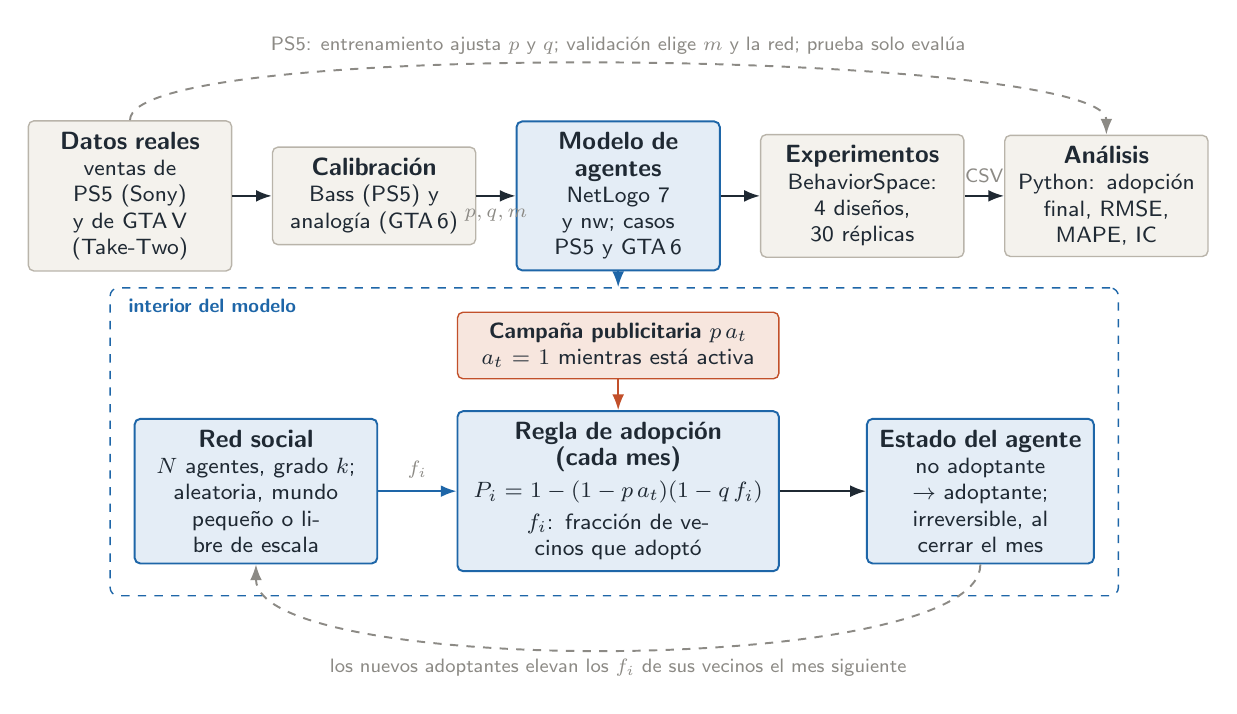
\begin{tikzpicture}[
  font=\footnotesize, text=tinta,
  caja/.style={draw=borde, line width=0.5pt, rounded corners=2pt, fill=white, align=center, inner sep=4pt, minimum height=11mm},
  etapa/.style={caja, fill=claro, text width=23mm},
  nucleo/.style={caja, fill=acentoclaro, draw=acento, line width=0.7pt},
  flecha/.style={-{Latex[length=2mm]}, line width=0.7pt, draw=tinta},
  nota/.style={font=\scriptsize, text=gris, align=center},
]

% ---------- fila superior: flujo de trabajo
\node[etapa] (datos) at (0,0) {\textbf{\small Datos reales}\\ventas de PS5 (Sony) y de GTA\,V (Take-Two)};
\node[etapa] (calib) at (3.1,0) {\textbf{\small Calibración}\\Bass (PS5) y analogía (GTA\,6)};
\node[etapa, fill=acentoclaro, draw=acento, line width=0.7pt] (abm) at (6.2,0) {\textbf{\small Modelo de agentes}\\NetLogo 7 y nw; casos PS5 y GTA\,6};
\node[etapa] (exp) at (9.3,0) {\textbf{\small Experimentos}\\BehaviorSpace: 4 diseños, 30 réplicas};
\node[etapa] (ana) at (12.4,0) {\textbf{\small Análisis}\\Python: adopción final, RMSE, MAPE, IC};

\draw[flecha] (datos) -- (calib);
\draw[flecha] (calib) -- node[below=1pt, nota] {$p,q,m$} (abm);
\draw[flecha] (abm) -- (exp);
\draw[flecha] (exp) -- node[above=1pt, nota] {CSV} (ana);
\draw[flecha, draw=gris, dashed] (datos.north) to[out=90, in=90, looseness=0.22]
  node[above, nota, pos=0.5] {PS5: entrenamiento ajusta $p$ y $q$; validación elige $m$ y la red; prueba solo evalúa} (ana.north);

% ---------- interior del modelo
\node[nucleo, text width=28mm] (red) at (1.6,-3.75)
  {\textbf{\small Red social}\\$N$ agentes, grado $k$;\\aleatoria, mundo pequeño o libre de escala};
\node[nucleo, text width=38mm] (regla) at (6.2,-3.75)
  {\textbf{\small Regla de adopción (cada mes)}\\[2pt]$P_i = 1-(1-p\,a_t)(1-q\,f_i)$\\[2pt]$f_i$: fracción de vecinos que adoptó};
\node[nucleo, text width=26mm] (estado) at (10.8,-3.75)
  {\textbf{\small Estado del agente}\\no adoptante $\rightarrow$ adoptante; irreversible, al cerrar el mes};
\node[caja, fill=terracotaclaro, draw=terracota, text width=38mm, minimum height=8mm] (campana) at (6.2,-1.9)
  {\textbf{Campaña publicitaria} $p\,a_t$\\$a_t=1$ mientras está activa};

\draw[flecha, draw=terracota] (campana) -- (regla);
\draw[flecha, draw=acento] (red) -- node[above=1pt, nota] {$f_i$} (regla);
\draw[flecha] (regla) -- (estado);
\draw[flecha, draw=gris, dashed] (estado.south) to[out=-90, in=-90, looseness=0.4]
  node[below, nota] {los nuevos adoptantes elevan los $f_i$ de sus vecinos el mes siguiente} (red.south);

\begin{scope}[on background layer]
  \node[draw=acento, dashed, rounded corners=3pt, line width=0.5pt, fill=white,
        fit=(red)(regla)(estado)(campana), inner xsep=3mm, inner ysep=3mm] (interior) {};
\end{scope}
\node[font=\scriptsize\bfseries, text=acento, anchor=west] at ($(interior.north west)+(1.2mm,-2.4mm)$) {interior del modelo};
\draw[flecha, draw=acento, dashed] (abm.south) -- (interior.north -| abm.south);

\end{tikzpicture}
\end{document}
